%%%%%%%%%%%%%%%%%%%%%%%%%%%%%%%%%%%%%%%%%%%%%%%%%%%%
\documentclass[fleqn,10pt,twocolumn]{SICE19}

%% パッケージ
%%\usepackage{Sotsuron_ptex} % タイトルページ用
\usepackage{fancyhdr}
\usepackage{indentfirst}
\usepackage[dvipdfmx]{graphicx}
\usepackage{subfigure} %Y subfigure環境用
\usepackage{amsmath} % 数式用
\usepackage{amssymb} % 数式用フォント
%\usepackage{color} %Y カラーのフォント用
\usepackage{booktabs}%表の罫線の太さ変更
\usepackage{multirow}%表の中の文字を複数行の中央に配置
\usepackage{comment}%複数行のコメントアウト用
\usepackage{bm}%ベクトル表示用
\usepackage{amsmath}%\begin{align}用
\usepackage{caption}%caption用
\usepackage{nidanfloat}%図ぶち抜きでbに挿入する用

%% その他変更パラメータ
\renewcommand{\baselinestretch}{1.1}
\renewcommand{\thefootnote}{\dag\arabic{footnote}} % 脚注番号表記
\graphicspath{{./figure/}} %図のパス指定
\usepackage{subfigure} %Y subfigure環境用
\usepackage{here}%Hによって図の位置強制出力
%% 図refの定義
\newcommand{\Figref}[1]{Fig.~\ref{#1}}
%% 表refの定義
\newcommand{\Tabref}[1]{Tab.~\ref{#1}}
%% 章refの定義
\newcommand{\Secref}[1]{Sec.~\ref{#1}}
%% 節refの定義
\newcommand{\Subsecref}[1]{Sec.~\ref{#1}}
%% 項refの定義
\newcommand{\Subsubsecref}[1]{Sec.~\ref{#1}}
%% 式refの定義
\newcommand{\Eqref}[1]{Eq.\,(\ref{#1})}

%% itemize1 環境
\newenvironment{itemize1}{\begin{list}{$\diamond$}{%
		\setlength{\topsep}{.5\normalbaselineskip}
		\setlength{\partopsep}{0\normalbaselineskip}
		\setlength{\parsep}{.1\normalbaselineskip}
		\setlength{\itemsep}{.2\normalbaselineskip}
		\setlength{\listparindent}{1zw}
		\setlength{\rightmargin}{1zw}
	}}{\end{list}}

%% enumerate1 環境
\newcounter{mycount}
\newenvironment{enumerate1}{\begin{list}{}{%
		\usecounter{mycount}
		\renewcommand{\makelabel}{\hfill(\arabic{mycount})}
		\setlength{\topsep}{.5\normalbaselineskip}
		\setlength{\partopsep}{0\normalbaselineskip}
		\setlength{\parsep}{.1\normalbaselineskip}
		\setlength{\itemsep}{.2\normalbaselineskip}
		\setlength{\leftmargin}{3zw}
		\setlength{\itemindent}{0zw}
		\setlength{\labelsep}{.5zw}
		\setlength{\labelwidth}{\leftmargin}
		\addtolength{\labelwidth}{-\itemindent}
		\addtolength{\labelwidth}{-\labelsep}
		\setlength{\listparindent}{1zw}
		\setlength{\rightmargin}{1zw}
	}}{\end{list}}

%%bibtexの環境
%\bibliographystyle{jplain} %Y 著者順の名前順に参考文献を並び変える
\bibliographystyle{junsrt} %Y 引用順に参考文献を並び変える

\title{Application of Compressed Sensing to Measurement of\\
       Methane Gas Distribution}

\author{Michiya Inagaki${}^{1\dagger}$, Haruka Matsukura${}^{1}$, Daisuke Iwai${}^{1}$ and Kosuke Sato${}^{1}$}
% The dagger symbol indicates the presenter.
\speaker{Michiya Inagaki}

\affils{${}^{1}$Graduate School of Engineering Science, Osaka University, Osaka, Japan\\
(Tel: +81-6-6850-6372; E-mail: inagaki@sens.sys.es.osaka-u.ac.jp)\\
}
\abstract{%
In waste landfill sites, monitoring of methane gas is essential for management of waste landfill sites and countermeasures against global warming. In general, the chamber method is used to monitor methane gas. In order to perform the chamber method, it is necessary to specify the gas sources position. It is effective to measure the gas distribution to identify the gas sources position. At present, a method using an optical-based gas sensor has been proposed to measure the gas distribution. However, this method requires a vast number of measurement data for reconstruction of gas distribution. Therefore, in this research, we proposed a method to reduce the number of required measurement data by applying compressed sensing to the conventional gas distribution reconstruction algorithm. As a result of reconstructing the gas distribution for fewer measurement data than usual, the reconstruction result with fewer artifacts was obtained in the proposed method than in the conventional method.}

\keywords{%
Gas sensing, Gas distribution map, Tomography, Compressed sensing.
}

\begin{document}

\maketitle

%-----------------------------------------------------------------------

\section{Introduction}\label{sec:intro}

Methane gas is a flammable gas and mixes with air to form an explosive mixture, which is an obstacle for waste landfill sites management and site reuse. It is reported in \cite{ref1} that methane gas leaks occur frequently even in waste landfill sites that have been closed for decades. Monitoring data of methane gas, which is an indicator of stabilization of waste landfill sites, is essential for securing the safety of waste landfill sites and surrounding areas. Also, gas monitoring from the viewpoint of global warming is regarded as important. Landfill gas composed of methane gas and carbon dioxide discharged from waste landfill sites accounts for 2\% of the total greenhouse gas released by human activity\cite{ref23}.

In waste landfill sites, in general, the chamber method is used to monitor methane gas\cite{ref24}. The chamber method is a method of calculating the release flux from the concentration change of the gas accumulated in the chamber covered on the soil covering surface. In order to perform the chamber method, it is necessary to specify the position of the gas sources. It is effective to measure the gas distribution to identify the gas sources position. As a research of gas distribution measurement, Trincavelli et al. proposed a gas distribution mapping (GDM) algorithm that performs gas measurement using an optical-based gas sensor and reconstructs the gas distribution from multiple measurement data\cite{ref9}. However, this method has a problem that an enormous number of measurement data are required to reconstruct the gas distribution.

Therefore, in this research, we applied compressed sensing to the conventional gas distribution reconstruction algorithm, GDM algorithm, and attempted to reduce the number of measurement data required for reconstruction of gas distribution. This aimed to improve the efficiency of gas distribution measurement work using an optical-based gas sensor.


\section{PROPOSED METHODS}\label{sec:proposed_methods}
\subsection{Measuring device}\label{subsec:system}
The measuring device is shown in \Figref{fig:robot}. In this measuring device, a biaxial scanning laser methane detector was mounted on a mobile robot, enabling movement of measurement positions. The biaxial scanning laser methane detector is a device in which a laser methane detector (Laser Methane mini SA3C32B, Tokyo Gas Engineering Solutions Corporation), hereinafter referred to as LMm, was mounted on a pan tilt unit (PTU-E46, FLIR), hereinafter referred to as PTU. By controlling the angle of the PTU, the biaxial scanning laser methane detector can irradiate the measurement laser of LMm in arbitrary up, down, right and left directions. We reconstruct the gas distribution by applying algorithms that incorporate compressed sensing into the GDM algorithm, using the measured values of the LMm and the control angle of the PTU.

\begin{figure}[h]
\begin{center}
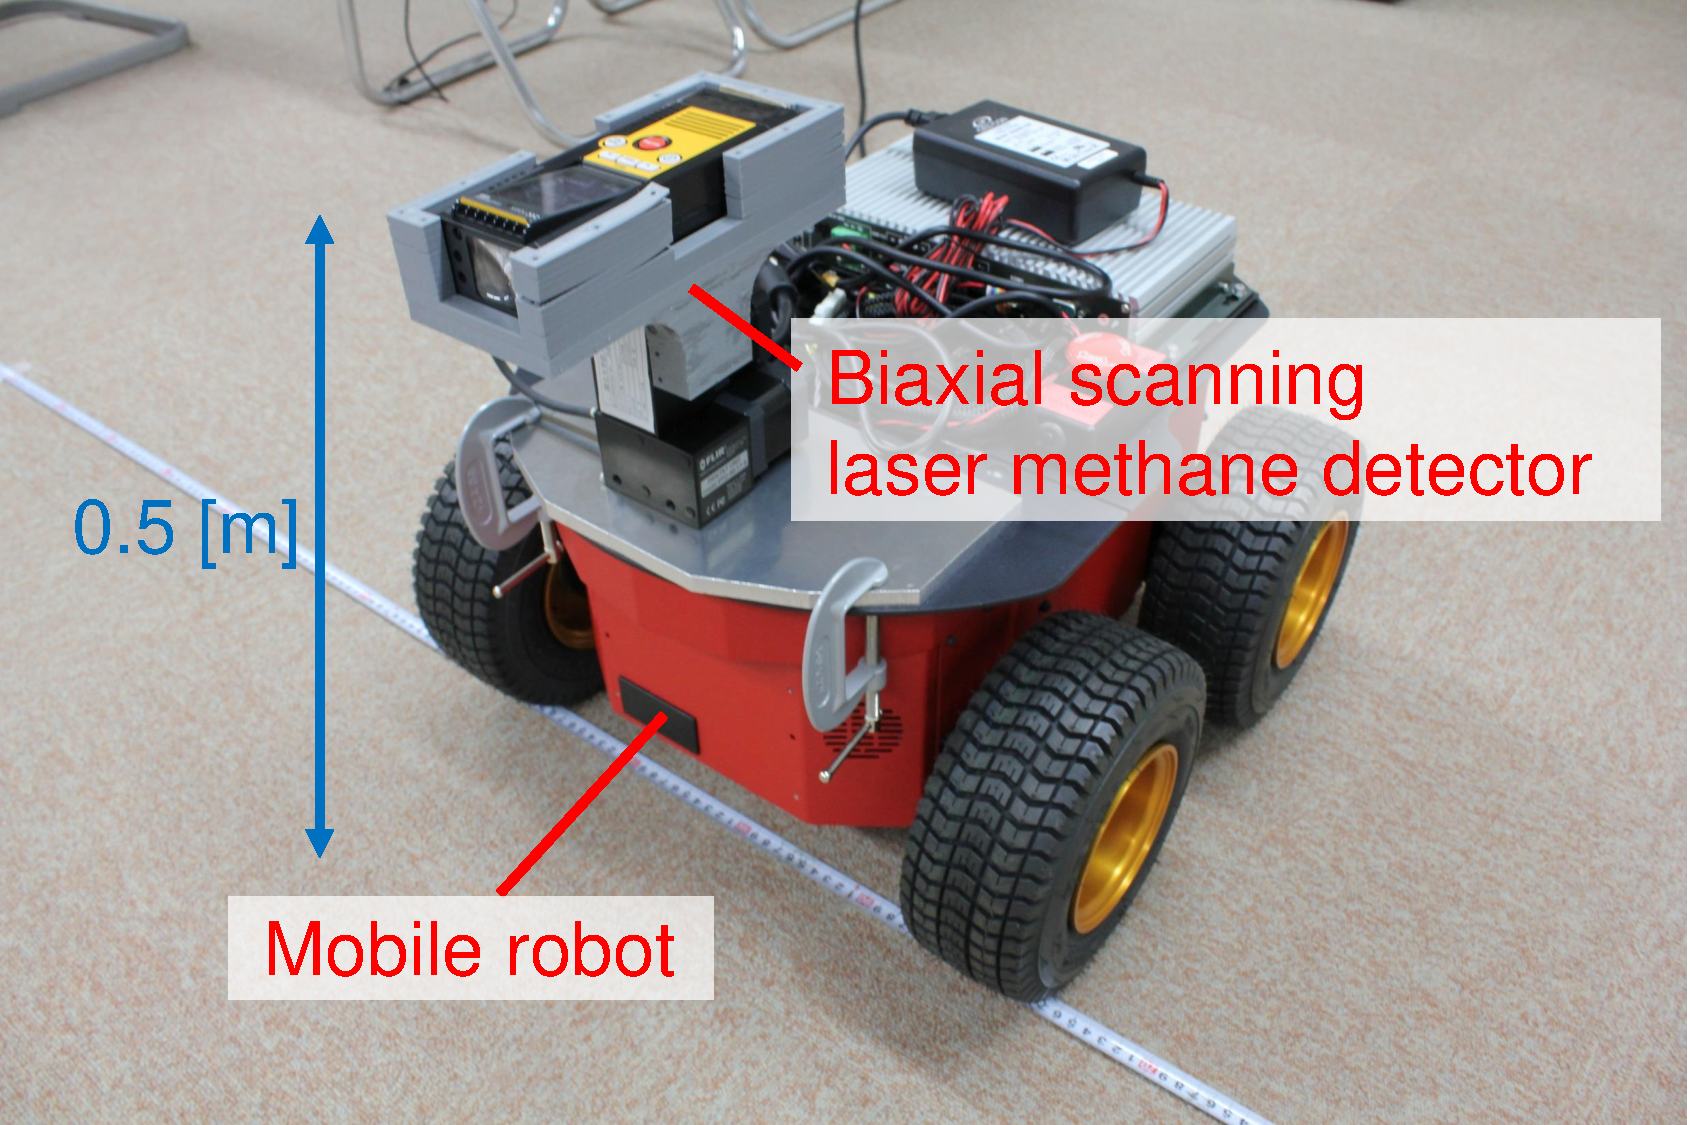
\includegraphics[width=70mm]{robot.pdf}
\caption{\label{fig:robot} Measuring device}
\end{center}
\end{figure}


\subsection{Gas distribution reconstruction algorithm applying compressed sensing}\label{subsec:algorithm}
The measured value of LMm is the methane column density [ppm · m], which is the integrated value of the gas concentration along the optical path of the laser. Therefore, it is not possible to obtain the density of each point on the optical path from the measured value. In order to acquire the concentration at each point in the mapping target region as the gas distribution, it is necessary to perform tomographic calculation based on the methane column density.

In this research, we proposed an algorithm applying compressed sensing for tomographic calculation based on GDM algorithm of Trincavelli et al.

As the first step of the algorithm, the mapping target area is divided into cells of virtual cubic lattice. In this algorithm, gas distribution is reconstructed by obtaining the concentration in each cell. Also assume that the concentration in each cell is uniform. Therefore, the size of one cell is the resolution of the gas distribution map. When the measured value of LMm is divided by the cells of the cubic lattice, it can be expressed as following equation:

\begin{eqnarray}
  \label{eq:splitop_1}
  y = \sum_{i=1}^N a_ix_i + \epsilon
\end{eqnarray}

\noindent
where $y$ is the LMm reading, $N$ is the number of cells, $a_i$ is the distance travelled by the laser in cell $i$, $x_i$ is the gas concentration in cell $i$, and $\epsilon$ is a measurement noise term. A conceptual diagram showing \Eqref{eq:splitop_1} in two dimensions for simplicity is shown in \Figref{fig:splitOP}.

\begin{figure}[h]
\begin{center}
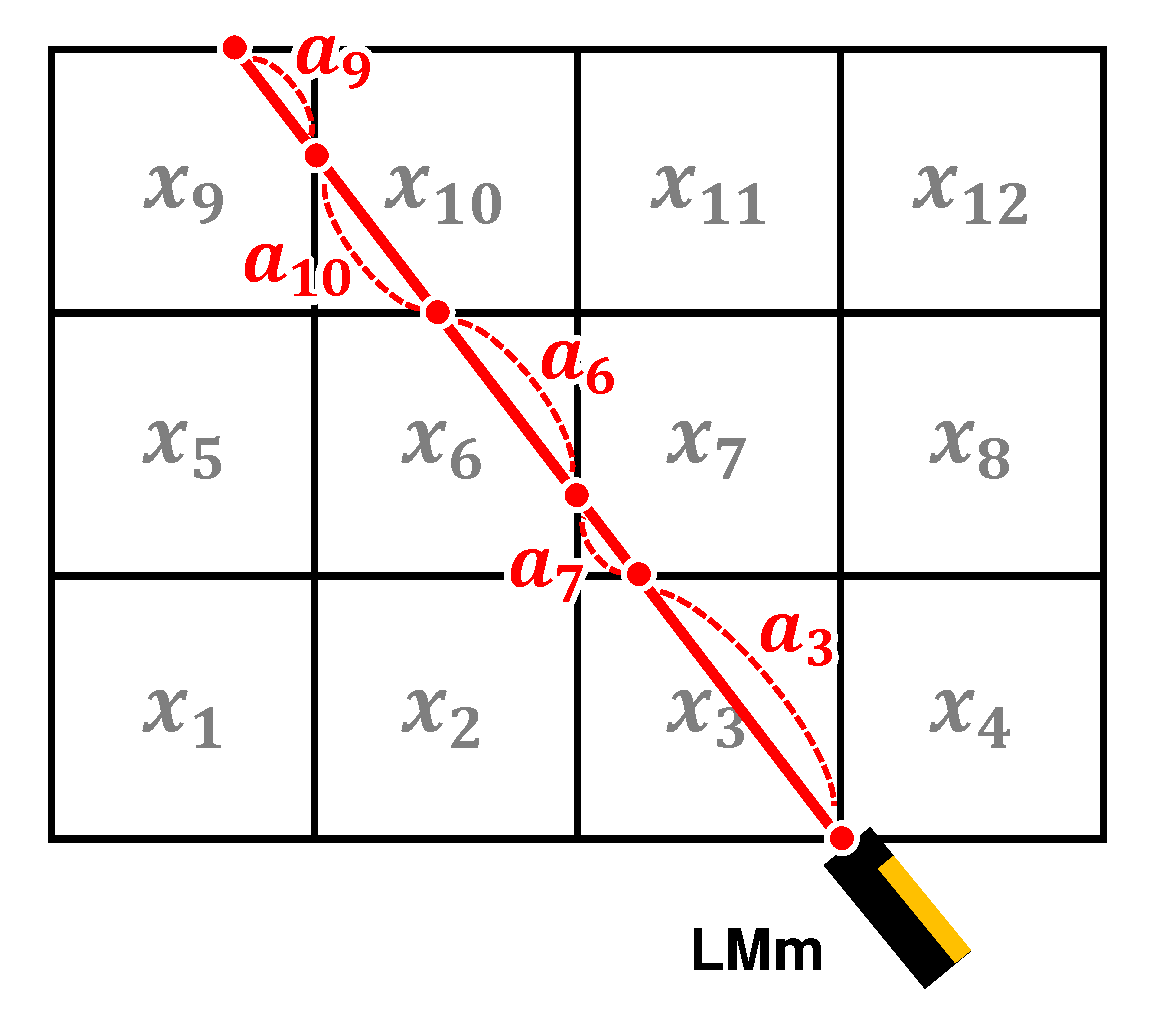
\includegraphics[width=65mm]{new_SplitOP}
\caption{\label{fig:splitOP} Conceptual diagram showing \Eqref{eq:splitop_1} in a simple two-dimensional manner.  The red line represents the optical path of the laser, in this case the measured value of LMm is divided by $y=a_{3}x_{3}+a_{6}x_{6}+a_{7}x_{7}+a_{9}x_{9}+a_{10}x_{10}+\epsilon$.
}
\end{center}
\end{figure}

Given a set of $M$ measured values, \Eqref{eq:splitop_1} can be expressed as following matrix equation:

\begin{eqnarray}
  \label{eq:splitop_2}
  \bm{y} = \bm{A}\bm{x} + \epsilon\bm{1}
\end{eqnarray}

\noindent
where $\bm{y}$ is the column vector of length $M$ that contains all the measurement values, $\bm{A}$ is the matrix of dimensions $M$$\times$$N$ that contains the laser distance in each measurement divided by cells, $\bm{x}$ is the column vector of length $N$ that contains the concentration values of the cells, $\bm{1}$ is a column vector of ones of length $M$. The problem of reconstructing the gas distribution from the measured values of LMm can be formulated as a problem for finding the gas concentration vector $\bm{x}$ in \Eqref{eq:splitop_2}.

Here, by applying compressed sensing\cite{ref25}, we tried to restore the gas concentration vector $\bm{x}$ from few observations. Compressed sensing deals with the problem that an unknown $N$-dimensional vector $\bm{x}$ is linearly transformed using an $M$$\times$$N$ matrix $\bm{A}$ as in \Eqref{eq:splitop_2}. Also, $\bm{y}$ is a known $M$-dimensional vector. At this time, restoring the unknown $N$-dimensional vector $\bm{x}$ from the lower dimensional $M$-dimensional vector $\bm{y}$ (in many cases, $M$$<$$N$) is a basic problem setting of compressed sensing.

\Eqref{eq:splitop_2} is a simultaneous linear equation, and generally, if the number of unknowns is larger than the number of equations, solutions can not be uniquely determined. However, when it is possible to assume that the unknown vector $\bm{x}$ is sparse, it is known that a solution can be successfully solved by solving following minimization problem by utilizing the property that the L1 norm easily holds a sparse solution.

\begin{eqnarray}
  \label{eq:CS_2}
  \begin{aligned}
    & \underset{{\bm x}} {\text{minimize}} &&\frac{1}{2\lambda}\|\bm{y}-\bm{A}\bm{x}\|_2^2+\|\bm{x}\|_1\\
  \end{aligned}
\end{eqnarray}

\noindent
where $\lambda$ is a parameter related to the sensitivity of noise. In general, when noise intensity is high and $\bm{y}$'s reliability is low, $\lambda$ is set to a large value. Conversely, when $\bm{y}$ is trusted, $\lambda$ is set to be small.

However, in gas distribution reconstruction algorithm, the unknown vector $\bm{x}$ to be found is the value of the gas concentration in each cell when the mapping target region is divided by the cells of the cubic lattice. Since the gas has a property of diffusing in a wide range, there is no cell having a gas concentration of 0, and it is considered that the vector $\bm{x}$ itself representing the gas concentration does not have sparsity. Therefore, a linear transformation $\bm{B}$ in the vector $\bm{x}$ is applied to convert it into a sparsity vector $\bm{z}$ as following matrix equation:

\begin{eqnarray}
  \label{eq:CS_3}
  \bm{z} = \bm{B}\bm{x}
\end{eqnarray}

\noindent
In this research, the Fourier transform is used as the linear transformation $\bm{B}$. When the transformation of \Eqref{eq:CS_3} is performed, the minimization problem to be solved is as following minimization problem:

\begin{eqnarray}
  \label{eq:CS_4}
  \begin{aligned}
    & \underset{{\bm z}} {\text{minimize}} &&\frac{1}{2\lambda}\|\bm{y}-\bm{A}\bm{B^{-1}}\bm{z}\|_2^2+\|\bm{z}\|_1\\
  \end{aligned}
\end{eqnarray}

\noindent
 Note that $\bm{B^{-1}}$ represents the inverse transformation of the linear transformation $\bm{B}$, which corresponds to the inverse Fourier transform in this case. The sparse vector $\bm{z}$ is obtained by solving the minimization problem of \Eqref{eq:CS_4}, and the gas concentration vector $\bm{x}$ is obtained by applying the inverse Fourier transform to the vector $\bm{z}$. FISTA (Fast iterative shrinkage-thresholding algorithm) which is a sequential solution was used as an algorithm for solving \Eqref{eq:CS_4}.


\section{EXPERIMENTAL SETUP}\label{sec:env}
The schematic diagram of the experiment is shown in \Figref{fig:env_img}. This experiment was conducted in an indoor environment where wind influence is small. The measurement area was a region of 2.0 × 2.0 × 0.6 [m], and measurement was carried out by scanning while irradiating LMm laser at intervals of 0.2 [m]. The installation position of the measuring device was set on a straight line 0.6 [m] before the measurement area. When the scanning from one position was completed, the device was shifted 0.2 [m] laterally and scanning the measurement area again. In this experiment, the number of measurement points to be scanned from one position was 121 points and the installation position of the device was 11 positions. Therefore, the total number of measurement data was 1,331.

\begin{figure}[h]
\begin{center}
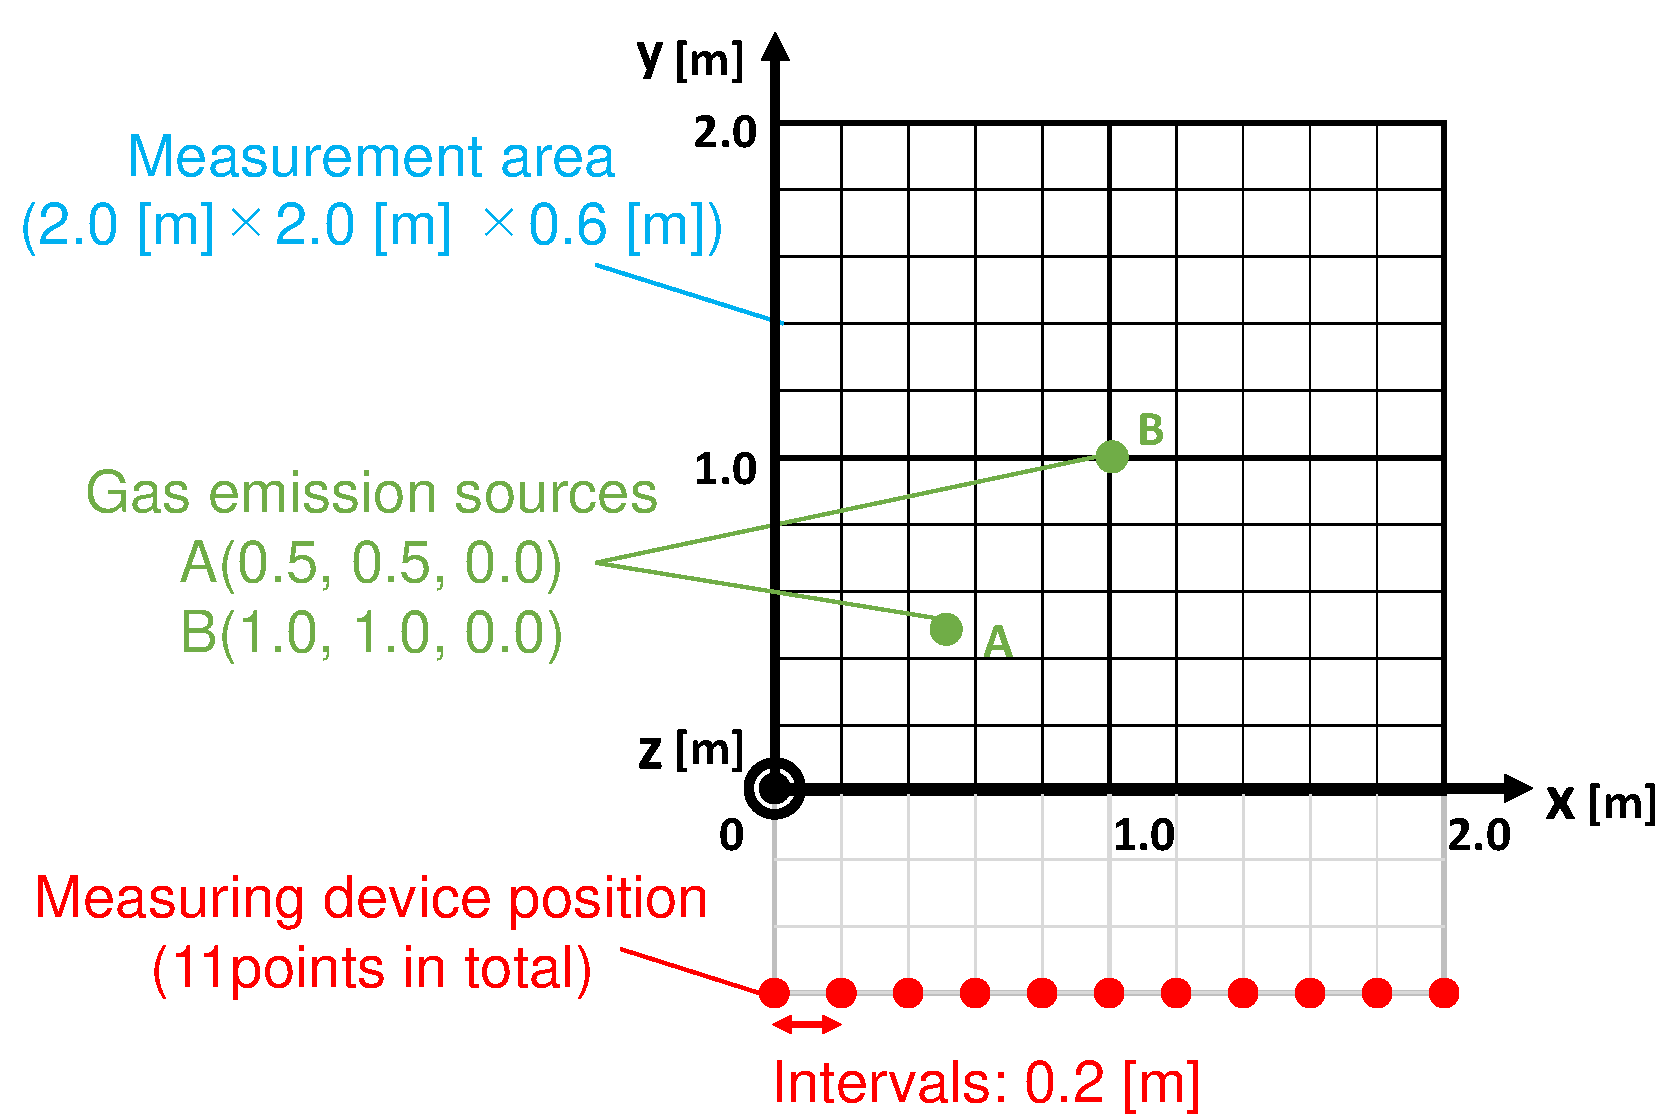
\includegraphics[width=80mm]{env_image.pdf}
\caption{\label{fig:env_img} Schematic diagram of experiment environment}
\end{center}
\end{figure}

The measurement time was about 3 minutes from one measuring device position, and the total time required for the measurement including the movement time of the installation position of the device was about 40 minutes.

As shown in \Figref{fig:env_img}, when the left front of the measurement area plane is the origin, the lateral direction is the x-axis, the longitudinal direction is the y-axis, and vertical direction is the z-axis, the gas emission source was arranged at  A:(x, y, z)[m]=(0.5, 0.5, 0.0), B:(x, y, z)[m]=(1.0, 1.0, 0.0). Methane gas was supplied to two gas emission sources through a tube with an inner diameter of 5 [mm] which was bifurcated from one gas cylinder and discharged in the positive direction of the x-axis from each tube openings. The methane gas concentration in the gas cylinder was 3\%, and the flow rate was 5 [L/min].

The gas distribution mapping area was a region with a width of 2.0 [m], a depth of 2.6 [m] (2.0 [m] of the measurement area + 0.6 [m] from the device installation position to the measurement area) and a height of 0.6 [m]. The size of the cell which is the resolution of the map was 0.2 × 0.2 × 0.2 [m]. Therefore, the total number of cells in the map was 390.


\section{RESULT}\label{sec:res}
As the data for applying the compressed sensing, measurement data from 2 positions at both ends out of the measurement data at 11 positions is used. The number of measurement data for 11 positions and 2 positions was 1,331 and 242 respectively. Since the total number of cells in the map was 390, the number of unknowns to be found exceeds the number of equations in \Eqref{eq:splitop_2}. Also, if converting the measurement data count from 1,331 points to 242 points into measurement time, we can reduce the time taken to take about 40 minutes to about 7 minutes.

 The result of applying the GDM algorithm using 1331 measurement data as a result close to the true value gas distribution is shown in \Figref{fig:11point_NP}. The results of applying the GDM algorithm using 242 measurement data is shown in \Figref{fig:2point_NP}. The results of applying compressed sensing to the GDM algorithm using the same 242 measured data is shown in \Figref{fig:2point_CS}. As the density value varies depending on the number of iterations of calculation, comparison was made focusing on the approximate shape of the distribution, not the density value.

\begin{figure}[h]
\begin{center}
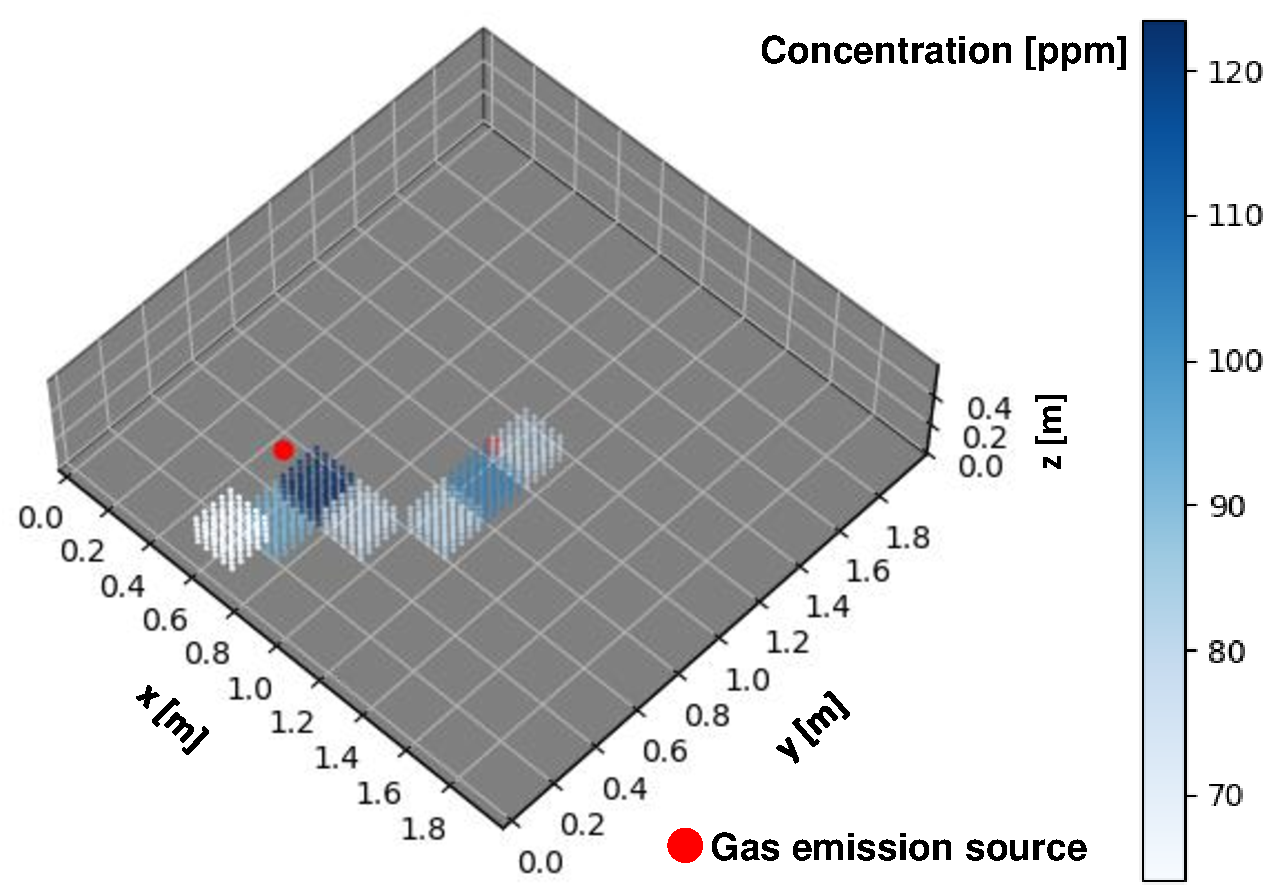
\includegraphics[width=80mm]{11point_NP.pdf}
\caption{\label{fig:11point_NP} Results of applying the GDM algorithm (Top 1.8\% high concentration cell, The number of data: 1,331)}
\end{center}
\end{figure}

\begin{figure}[h]
\begin{center}
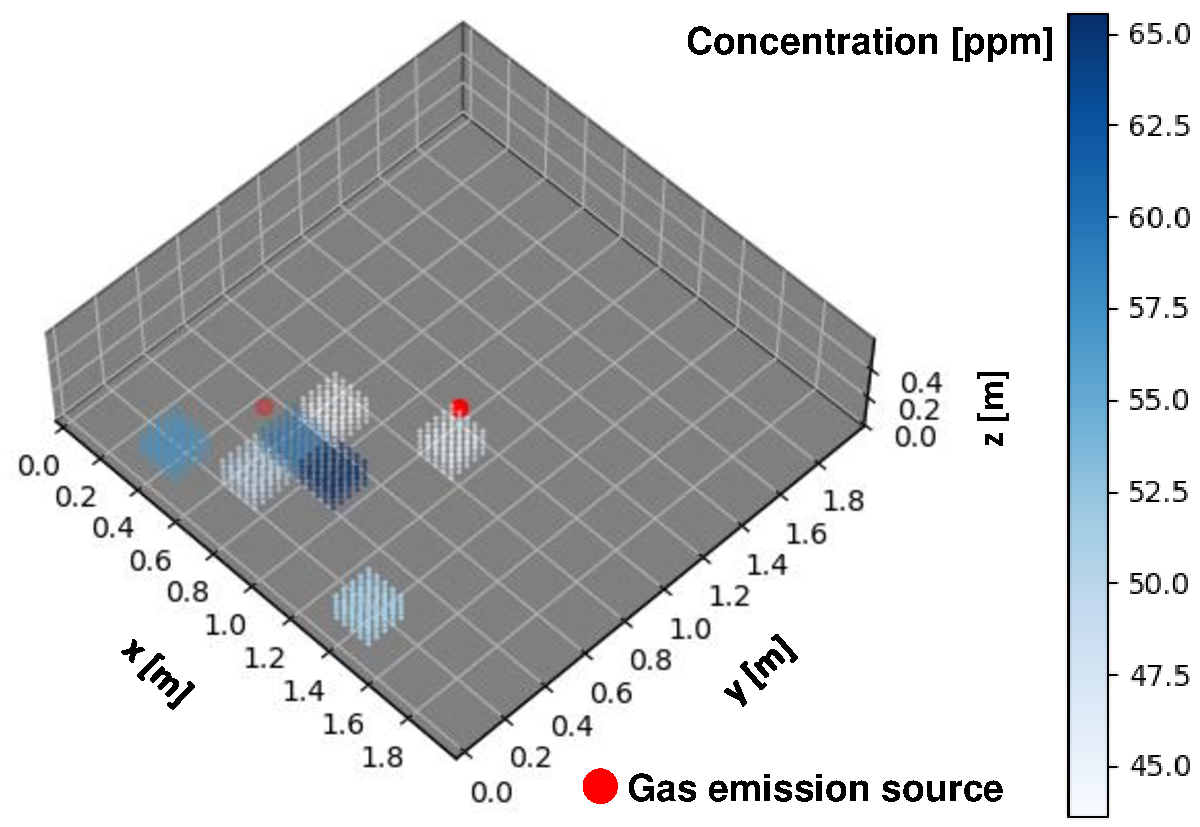
\includegraphics[width=80mm]{2point_NP.pdf}
\caption{\label{fig:2point_NP} Results of applying the GDM algorithm (Top 1.8\% high concentration cell, The number of data: 242)}
\end{center}
\end{figure}

\begin{figure}[h]
\begin{center}
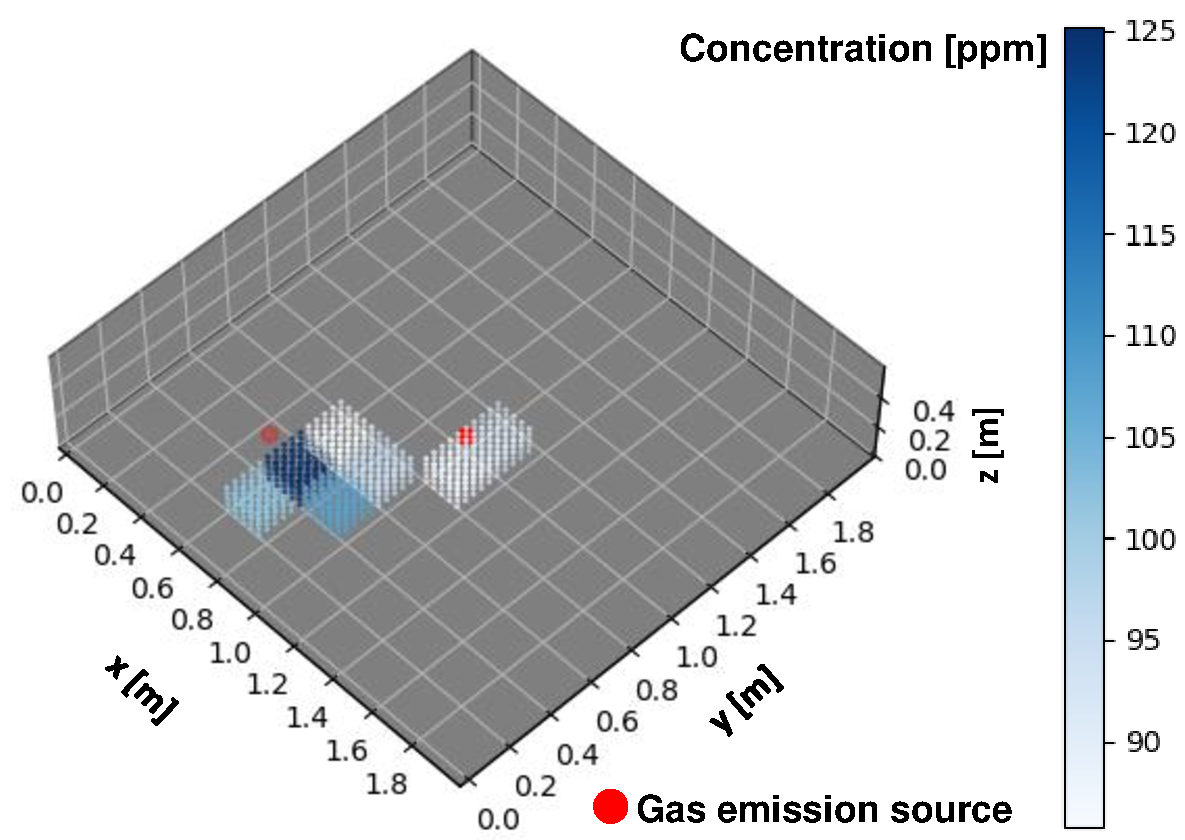
\includegraphics[width=80mm]{2point_CS.pdf}
\caption{\label{fig:2point_CS} Results of applying the compressed sensing (Top 1.8\% high concentration cell, The number of data: 242, $\lambda=1.5$, FISTA iteration count:100)}
\end{center}
\end{figure}


In \Figref{fig:2point_NP}, cells with high concentrations considered to be noise are distributed at positions away from the gas emission sources. In particular, paying attention to the gas emission source in front of the left in \Figref{fig:2point_NP}, the cell with the highest concentration is not the cell immediately adjacent to the gas emission source but the cell next to the next gas emission source. It can not be said that the distribution is correctly reconstructed even if this is compared with \Figref{fig:11point_NP} which is a reconstructed map using 1,331 measured data.

On the other hand, in \Figref{fig:2point_CS}, it can be seen that the characteristics of distribution are captured because cells with high concentration are concentrated near the gas emission sources and artifacts are small. It can be said that the distribution close to the true distribution is reconstructed even in comparison with \Figref{fig:11point_NP}.


\section{CONCLUTION}\label{sec:conclition}
In this research, we tried to reduce the number of measurement data required for reconstruction of gas distribution by applying compressed sensing to the conventional gas distribution reconstruction algorithm. A measurement experiment was carried out and it was found that the characteristics of the distribution could be captured for the case of applying the compressed sensing rather than the GDM algorithm for the small measurement data. From this result, it was suggested that application of compressed sensing to the GDM algorithm could reduce the number of measurement data which can make the work of gas distribution measurement more efficient.

In this research, Fourier transform was used as a transformation function giving sparsity to the gas concentration vector of \Eqref{eq:CS_3}. However, appropriate transformation functions will be considered in the future. In addition, the value of $\lambda$ in \Eqref{eq:CS_2} and the number of iterations of FISTA to solve \Eqref{eq:CS_4} was determined empirically, and examination of indices for determining these parameters is also a future subject.

Also, since it was not possible to obtain gas distribution data that is a true value with respect to measurement data applied with compressed sensing this time, the usefulness of compressed sensing had not been quantitatively verified. Therefore, we will consider evaluating compressed sensing using numerical simulation in the future.



%%%%%%%%%%%%%%%%% BIBLIOGRAPHY IN THE LaTeX file !!!!! %%%%%%%%%%%%%%%%%%%%%%
\begin{thebibliography}{9}

\bibitem{ref1}
Victor Hernandez Bennetts, Achim J. Lilienthal, Patrick P. Neumann and Marco Trincavelli, ``Mobile robots for localizing gas emission sources on landfill sites: is bio-inspiration the way to go?'',
{\it Frontiers in neuroengineering}, Vol. 4, pp. 20, 2012.

\bibitem{ref23}
J. Bogner, M. A. Ahmed, C. Diaz, A. Faaij, Q. Gao, S. Hashimoto, K. Mareckova, R. Pipatti, and T. Zhang, ``Climate Change 2007: Mitigation. Contribution of Working Group III to the Fourth Assessment Report of the Intergovernmental Panel on Climate Change''
{\it Waste Management}, pp. 595--596, 2007.

\bibitem{ref24}
Gunnar BÖrjesson, Åsa Danielsson, and Bo H. Svensson, ``Methane Fluxes from a Swedish Landfill Determined by Geostatistical Treatment of Static Chamber Measurements''
{\it Environmental Science \& Technology}, Vol.34, No.18, pp. 4044--4050, 2000.

\bibitem{ref9}
Marco Trincavelli, Victor Hernandez Bennetts, and Achim J Lilienthal, ``A least squares approach for learning gas distribution maps from a set of integral gas concentration measurements obtained with a TDLAS sensor''
{\it IEEE Sensors}, 2012.

\bibitem{ref25}
Marco F. Duarte and Yonina C. Eldar, ``Structured Compressed Sensing: From Theory to Applications''
{\it IEEE Transactions on Signal Processing}, Vol.59, No.9, pp. 4053--4085, 2011.


\end{thebibliography}

\end{document}
